% Source - https://tex.stackexchange.com/a/761452
\documentclass[tikz,border=5pt]{standalone}
\usetikzlibrary{nfold}
\makeatletter
\tikzset{offset/.code=\tikz@addmode{\pgfgetpath\tikz@temp\pgfsetpath\pgfutil@empty\pgfoffsetpath\tikz@temp{#1}}}
\makeatother
\begin{document}
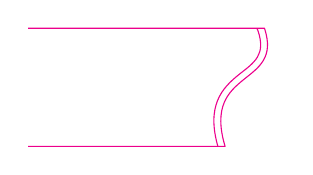
\begin{tikzpicture}[
  line join=round,
  double path/.style={insert path={.. controls ++(.25,-.75) and ++(-.3,1) .. (doubleend)}}
]
\path (0  , 1.5) coordinate (start)
    ++(3  , 0  ) coordinate (doublestart)
    ++(-.5,-1.5) coordinate (doubleend)
      (0  , 0  ) coordinate (end)
  (doublestart) [double path] coordinate[pos=-.1] (doublestart-early)
;
\draw[magenta]
  (start) -- (doublestart) [double path] -- (end)
  [path picture={
      \draw (doublestart-early) -- (doublestart) [offset=-2.5pt, double path];
  }]
  ;
\end{tikzpicture}
\end{document}

% path picture 选项应用于路径且 <code> 非空时，将发生以下情况：在完成由 fill、pattern 和 shade 选项引发的所有其他"填充"操作后，会开启一个局部作用域，并将该路径临时设置为裁剪路径。随后执行 <code> 代码，此时可绘制任意内容。接着局部作用域结束，若已指定 draw 选项，则可能对路径进行描边。